\documentclass[]{elsarticle} %review=doublespace preprint=single 5p=2 column
%%% Begin My package additions %%%%%%%%%%%%%%%%%%%
\usepackage[hyphens]{url}
\usepackage{lineno} % add
\providecommand{\tightlist}{%
  \setlength{\itemsep}{0pt}\setlength{\parskip}{0pt}}

\bibliographystyle{elsarticle-harv}
\biboptions{sort&compress} % For natbib
\usepackage{graphicx}
\usepackage{booktabs} % book-quality tables
%% Redefines the elsarticle footer
%\makeatletter
%\def\ps@pprintTitle{%
% \let\@oddhead\@empty
% \let\@evenhead\@empty
% \def\@oddfoot{\it \hfill\today}%
% \let\@evenfoot\@oddfoot}
%\makeatother

% A modified page layout
\textwidth 6.75in
\oddsidemargin -0.15in
\evensidemargin -0.15in
\textheight 9in
\topmargin -0.5in
%%%%%%%%%%%%%%%% end my additions to header

\usepackage[T1]{fontenc}
\usepackage{lmodern}
\usepackage{amssymb,amsmath}
\usepackage{ifxetex,ifluatex}
\usepackage{fixltx2e} % provides \textsubscript
% use upquote if available, for straight quotes in verbatim environments
\IfFileExists{upquote.sty}{\usepackage{upquote}}{}
\ifnum 0\ifxetex 1\fi\ifluatex 1\fi=0 % if pdftex
  \usepackage[utf8]{inputenc}
\else % if luatex or xelatex
  \usepackage{fontspec}
  \ifxetex
    \usepackage{xltxtra,xunicode}
  \fi
  \defaultfontfeatures{Mapping=tex-text,Scale=MatchLowercase}
  \newcommand{\euro}{€}
\fi
% use microtype if available
\IfFileExists{microtype.sty}{\usepackage{microtype}}{}
\usepackage[left=2.5cm,right=2.5cm,top=2.5cm,bottom=2.5cm]{geometry}
\usepackage{longtable}
\usepackage{graphicx}
% We will generate all images so they have a width \maxwidth. This means
% that they will get their normal width if they fit onto the page, but
% are scaled down if they would overflow the margins.
\makeatletter
\def\maxwidth{\ifdim\Gin@nat@width>\linewidth\linewidth
\else\Gin@nat@width\fi}
\makeatother
\let\Oldincludegraphics\includegraphics
\renewcommand{\includegraphics}[1]{\Oldincludegraphics[width=\maxwidth]{#1}}
\ifxetex
  \usepackage[setpagesize=false, % page size defined by xetex
              unicode=false, % unicode breaks when used with xetex
              xetex]{hyperref}
\else
  \usepackage[unicode=true]{hyperref}
\fi
\hypersetup{breaklinks=true,
            bookmarks=true,
            pdfauthor={},
            pdftitle={A reproducible journal article with RMarkdown: A building science template with examples for beginners based on the Elsevier journal format},
            colorlinks=true,
            urlcolor=blue,
            linkcolor=blue,
            pdfborder={0 0 0}}
\urlstyle{same}  % don't use monospace font for urls
\setlength{\parindent}{0pt}
\setlength{\parskip}{6pt plus 2pt minus 1pt}
\setlength{\emergencystretch}{3em}  % prevent overfull lines
\setcounter{secnumdepth}{5}
\usepackage{setspace}
\doublespacing
\usepackage[font={small}]{caption}
% Pandoc toggle for numbering sections (defaults to be off)
% Pandoc header
\usepackage{setspace}
\doublespacing
\usepackage[font={small}]{caption}


\usepackage[nomarkers]{endfloat}

\begin{document}
\begin{frontmatter}

  \title{A reproducible journal article with RMarkdown: A building science
template with examples for beginners based on the Elsevier journal
format}
    \author[CBE]{Paul Raftery\corref{c1}}
   \ead{p.raftery@berkeley.edu} 
   \cortext[c1]{Corresponding Author}
    \author[CBE]{Dana Miller}
  
  
    \author[Organization2]{Next contributor}
  
  
      \address[CBE]{Center for the Built Environment, UC Berkeley, 390 Wurster Hall,
Berkeley, CA, 94720, USA}
    \address[Organisation2]{Another organization, and their address}
  
  \begin{abstract}
  Enter the text for your abstract here. All data and analysis code in
  this template is publicly available at
  \url{https://github.com/CenterForTheBuiltEnvironment/rmd-example} and
  can be freely adapted and reused. Suggestions or pull requests to
  improve this template or create additional templates are welcome.
  \end{abstract}
  
 \end{frontmatter}

Keywords:\\
Keyword 1; Keyword 2; Keyword 3; Keyword 4; Keyword 5; Keyword 6 (max)

\pagebreak

\textbf{Highlights:}

\begin{itemize}
\tightlist
\item
  Add your 3 -5 highlights
\item
  As bulletpoints here
\item
  Making sure each is less than 85 characters in length
\end{itemize}

\textbf{Graphical Abstract}\\

\includegraphics{C:/Users/Dana/3_Professional/CBE/Reproducibility/cbe-rmd-example/Paper/SupplementaryMaterial/Images/Latex_logo.png}

\pagebreak

\section{Introduction}\label{introduction}

The purpose of this (very much work-in-progress) document is to provide
a complete R markdown template for an Elsevier journal submission (based
on the rticles repository Allaire et al.
(\protect\hyperlink{ref-rticles}{2017})), along with useful examples and
packages to improve usability for folks who are just starting out with
this workflow. The eventual intent is to capture minimal examples of the
common things that authors need to do when writing papers in R markdown;
provide examples of useful packages, workflows, and tools; and provide
solutions to common issues that folks encounter.

You may wish to have short sub-sections for:

\begin{itemize}
\tightlist
\item
  Terminology
\item
  Objectives
\end{itemize}

\section{\texorpdfstring{Methods (this is a `level 1
heading')}{Methods (this is a level 1 heading)}}\label{methods-this-is-a-level-1-heading}

\subsection{\texorpdfstring{Markdown (this is a `level 2
heading')}{Markdown (this is a level 2 heading)}}\label{markdown-this-is-a-level-2-heading}

This RMarkdown document is a special type of interactive document that
can contain both code chunks (in R, python, or other languages), and
text written in a format called Markdown. Here are some examples of how
to format text with Markdown, and a
\href{https://www.rstudio.com/wp-content/uploads/2015/03/rmarkdown-reference.pdf}{link}
to an RMarkdown guide.

\subsubsection{Level 3 heading}\label{level-3-heading}

Here's how to \textbf{bold} or \emph{italicize} a piece of text. This is
how you do a bullet point list:

\begin{itemize}
\tightlist
\item
  First bullet
\item
  Second bullet

  \begin{itemize}
  \tightlist
  \item
    A sub-bullet
  \item
    Another sub-bullet
  \end{itemize}
\end{itemize}

Or an ordered option:

\begin{enumerate}
\def\labelenumi{\arabic{enumi}.}
\tightlist
\item
  Item 1
\item
  Item 2

  \begin{itemize}
  \tightlist
  \item
    Item 2a
  \item
    Item 2b
  \end{itemize}
\end{enumerate}

\subsection{Tables}\label{tables}

Here is an example of a table created from the .csv file in the
\texttt{SupplementaryMaterial/Data}folder using the \texttt{gt} package
from RStudio. You can read more about \texttt{gt}
\href{https://github.com/rstudio/gt}{here}, and there's helpful examples
to further customize tables (eg with color, foototes, significant
figures, re-labeling columns, and more)
\href{https://github.com/allisonhorst/gt-awesome-tables}{here}.

\captionsetup[table]{labelformat=empty,skip=1pt}

\begin{longtable}{lrrc}
\caption*{
\large Example irises\\ 
\small Data on five randomly selected irises\\ 
} \\ 
\toprule
iris\_class & sepal\_length & petal\_length & petal\_length\_level \\ 
\midrule
Iris-virginica & 6.4 & 5.5 & High \\ 
Iris-virginica & 6.9 & 5.4 & High \\ 
Iris-setosa & 4.4 & 1.3 & VeryLow \\ 
Iris-virginica & 7.7 & 6.7 & VeryHigh \\ 
Iris-versicolor & 5.0 & 3.3 & Medium \\ 
\bottomrule
\end{longtable}

\subsection{Cross-referencing}\label{cross-referencing}

This is how you refer to a figure in your text: Figure
\ref{fig:correlation}. Simply reference the title of the code chunk, and
ensure that the code chunk includes a figure caption.

\begin{figure}
\centering
\includegraphics{C:/Users/Dana/3_Professional/CBE/Reproducibility/cbe-rmd-example/Paper/SupplementaryMaterial/Images/Correlation.png}
\caption{\label{fig:correlation}Correlation. Source: XKCD, xkcd.com/552}
\end{figure}

\subsection{Calculations in text}\label{calculations-in-text}

The holy grail of markdown - doing all of your calculations in the same
file so you never need to worry about updating them after
someone\footnote{Often I'm the someone, sorry CBE grad students. Also,
  look, it's an example of a footnote!} asks you to make
changes\ldots{}. again! It's as easy as pi: 3.14. Incidentally,you can
selectively override the `global' options set at the beginning, to say
for example, show more decimals: 3.1416.

This is an example of outputing the result of a calculation that you
perform within a code chunk in the document somewhere prior to the
location where you first refer to it: 36.

\subsection{Citations}\label{citations}

Citing other literature is remarkably easy, just like this Coakley,
Raftery, \& Keane
(\protect\hyperlink{ref-coakleyReviewMethodsMatch2014}{2014}). This
citation key references the tag associated with an entry in
Bibliography.bib (a BibTex file). I've found it easiest to use Zotero to
manage my library of references and to generate the BibTex file, though
any software that creates a valid BibTex file should work fine. Zotero
allows you to create a `Collection' (or folder) that gathers together
all of the references used for a particular document. When combined with
with the Better BibTex plugin, that collection can be exported to a
BibTex file that is continually updated as you add or edit references in
that Collection. Better BibTex also puts the citation key - the text
after the `@' sybmbol in the .Rmd file - on the upper right of each
entry, which is convenient for adding citations.

There's not much else involved in citing, as the references list gets
built and formatted automatically based on the selected style. The only
other issue I've had to look around to solve was figuring out how to
combine multiple citations, which is easy when you know how. (Coakley et
al., \protect\hyperlink{ref-coakleyReviewMethodsMatch2014}{2014}; Zhai
et al., \protect\hyperlink{ref-zhaiHumanComfortPerceived2015a}{2015})

The instructions for installing BetterBibtex are
\href{https://retorque.re/zotero-better-bibtex/}{here}.

\subsubsection{Citing software}\label{citing-software}

It is also good practice to include citations not such for literature
like journal articles and reports, but also the software used in the
analysis. Many software packages have accompanying publications that can
be cited, and even if they don't it is important to attribute which
version and which software you used. Citing software helps to provide
credit for the creators and maintainors of the software and demonstrate
that people (like you!) are using the software, which is especially
important for open-source tools supported through public research
funding.

You can use the \texttt{greatful} package to quickly generate a list of
the packages for software used in an R project using the
\texttt{cite\_packages} function from \texttt{greatful}. There is an
additional function called \texttt{get\_citations} that generates the
Bibtex-formatted citations for each package. It's not elegant, but you
can use the first to list packages used, then generate the
\texttt{pkg-refs.bib} file (saved to
\texttt{/Paper/SuplementaryMaterial} by default in this template), copy
the content into your overall \texttt{Bibliography.bib} file for the
whole document, and then cite the packages in your document as you would
another source, eg by using \texttt{@base} for an in-text citation for
core R software before other packages are installed (also known as `base
R').

\begin{itemize}
\tightlist
\item
  base R - R Core Team (\protect\hyperlink{ref-base}{2018})
\item
  ggpmisc - Aphalo (\protect\hyperlink{ref-ggpmisc}{2016})
\item
  grateful - Rodriguez-Sanchez (\protect\hyperlink{ref-grateful}{2018})
\item
  gt - Iannone, Cheng, \& Schloerke (\protect\hyperlink{ref-gt}{2019})
\item
  here - Müller (\protect\hyperlink{ref-here}{2017})
\item
  knitr - Xie (\protect\hyperlink{ref-knitr}{2018})
\item
  tidyverse - Wickham (\protect\hyperlink{ref-tidyverse}{2017})
\item
  rticles - Allaire et al. (\protect\hyperlink{ref-rticles}{2017})
\item
  bookdown - Xie (\protect\hyperlink{ref-bookdown}{2016})
\item
  rmarkdown - Allaire et al. (\protect\hyperlink{ref-rmarkdown}{2018})
\end{itemize}

\subsection{Equations and math}\label{equations-and-math}

Here's a basic example inline \(example_{subscript} = \frac{D}{R}\), or
you display it on a whole line if needed. Google latex math cheat sheets
for more information.

\[\sum_{i=1}^{n}{x_i^2}\]

Here is another equation:

\[ CD_{rated} = \frac{4*Q}{\pi*D^2} = 2.0~m/s\]

\subsection{Other packages}\label{other-packages}

There are lots of packages that are useful for markdown docs and
customizing plots. We encourage you to search for these whenever you
encounter a new thing you need to do and to propose an addition to this
repository accordingly. Some examples to start: \texttt{ggExtra},
\texttt{gridExtra}, \texttt{RColorBrewer}, \texttt{ggrepel}\ldots{}

\subsection{Writing style}\label{writing-style}

This is a little off topic for an Rmd example but a convenient place to
remind our grad students about writing style. In almost all cases,
active voice is better than passive voice. Several psychological studies
show that the active voice is more easily understood by readers, and
that information is more accurately reported by authors when writing in
active voice. For example, research Klenbort \& Anisfeld
(\protect\hyperlink{ref-klenbortMarkednessPerspectiveInterpretation1974}{1974})
has shown that the ``active {[}voice{]} offers a neutral structure for
conveying information''. Authorship guides for highly regarded journals
often indicate a preference for the active voice instead of passive:

\begin{itemize}
\tightlist
\item
  Nature: ``Nature journals like authors to write in the active voice
  (`we performed the experiment\ldots{}') as experience has shown that
  readers find concepts and results to be conveyed more clearly if
  written directly.''(``Nature - How to write a paper,'' n.d.)
\item
  Science: ``Use active voice when suitable, particularly when necessary
  for correct syntax (e.g., `To address this possibility, we constructed
  a lZap library \ldots{},' not `To address this possibility, a lZap
  library was constructed\ldots{}').'' Ruben, 2012, \& Am
  (\protect\hyperlink{ref-rubenHowWriteScientist2012}{2012})
\end{itemize}

And, on top of all that, you also end up with less text if you write in
active voice, saving space for useful information and making it easier
for your readers to understand.

\subsubsection{A fun way to spot passive
voice:}\label{a-fun-way-to-spot-passive-voice}

If you can add the words `by zombies' (``A scary-easy way to help you
find passive voice!''
\protect\hyperlink{ref-ScaryeasyWayHelp2014}{2014}) to the end of the
sentence and the sentence still makes logical sense, then the sentence
is in passive voice. You can also switch on the grammar settings in
Microsoft Word's spelling and grammar checker and it will show up that
way.

How to fix it?

Change:

``These measurements are not quantitatively reported in the paper''
(\ldots{} by zombies)

To

``The paper does not quantitatively report these measurements''

Or even better, it's really the authors doing the reporting as the paper
is an inanimate object\ldots{}

``We do not quantitatively report these measurements''.

Change:

``Six different table and partition configurations were tested''
(\ldots{} by zombies)

To

``We tested six different table and partition configurations.''

\section{Results}\label{results}

\subsection{Scatter plot example}\label{scatter-plot-example}

Figure \ref{fig:irises} shows petal widths by iris type.

\begin{figure}[h]

{\centering 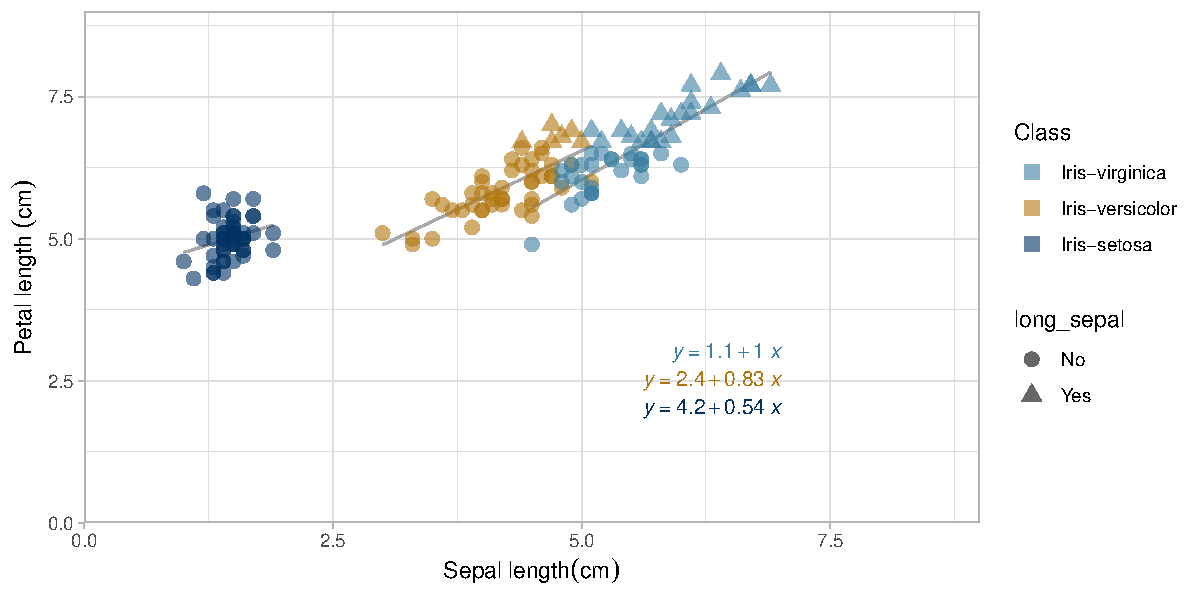
\includegraphics{Manuscript_files/figure-latex/irises-1} 

}

\caption{Petal and sepal lengths from iris dataset}\label{fig:irises}
\end{figure}

\subsection{Violin plot example}\label{violin-plot-example}

Figure \ref{fig:petalwidths} shows petal widths by iris type.

\begin{figure}[h]

{\centering 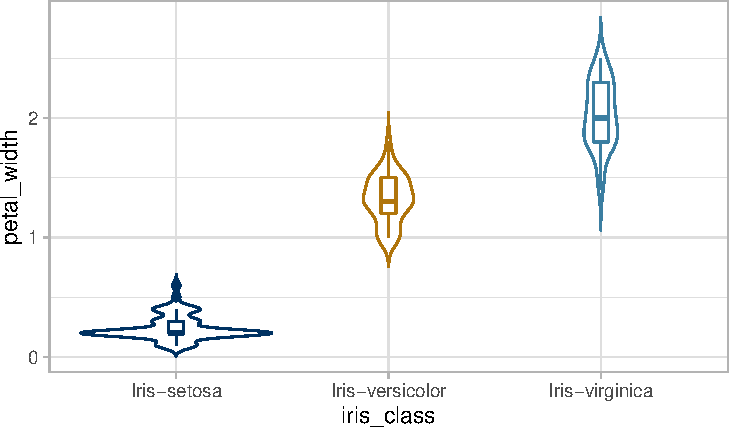
\includegraphics{Manuscript_files/figure-latex/petalwidths-1} 

}

\caption{Iris petal widths by species}\label{fig:petalwidths}
\end{figure}

\section{Discussion}\label{discussion}

\section{Limitations}\label{limitations}

It is important to include a discussion of limitations in any paper.
Some limitations of this template include:

\begin{itemize}
\tightlist
\item
  Whether or not figures are included inline with text appears to depend
  of the version of LaTeX the document is compiled with. Compiling on a
  computer where TinyTeX is installed (eg in the Binder associated with
  the reporsitory for this project on GitHub) will render the figures
  inline, whereas compiling the same document on a Windows computer with
  MikTeX installed does not
\item
  Does not include instructions on how to align figures
\end{itemize}

\section{Conclusion}\label{conclusion}

\section{Acknowledgements}\label{acknowledgements}

Don't forget to acknowledge the funder(s) with associated grant numbers
if required. The same goes for folks who significantly assisted you with
this paper but that are not authors. Eg ``Agency (grant number 12345)
supported this work, with cost share provided by the Center for the
Built Environment. We thank Person1 and Person2 for assistance with data
collection''

\section{Declaration of interest}\label{declaration-of-interest}

Descibe any relevant interests of the authors, particularly if there is
a link to the research that is relatively uncommon and could be
perceived as a conflict of interest. Otherwise : All authors declare no
conflict of interest.

\section*{References}\label{references}
\addcontentsline{toc}{section}{References}

\hypertarget{refs}{}
\hypertarget{ref-ScaryeasyWayHelp2014}{}
A scary-easy way to help you find passive voice! (2014). \emph{A
scary-easy way to help you find passive voice! \textbar{} Grammarly
Blog}.
https://www.grammarly.com/blog/a-scary-easy-way-to-help-you-find-passive-voice/.

\hypertarget{ref-rticles}{}
Allaire, J., R Foundation, Wickham, H., Journal of Statistical Software,
Xie, Y., Vaidyanathan, R., \ldots{} Yu, M. (2017). \emph{Rticles:
Article formats for r markdown}. Retrieved from
\url{https://CRAN.R-project.org/package=rticles}

\hypertarget{ref-rmarkdown}{}
Allaire, J., Xie, Y., McPherson, J., Luraschi, J., Ushey, K., Atkins,
A., \ldots{} Chang, W. (2018). \emph{Rmarkdown: Dynamic documents for
r}. Retrieved from \url{https://CRAN.R-project.org/package=rmarkdown}

\hypertarget{ref-ggpmisc}{}
Aphalo, P. J. (2016). \emph{Learn r ...as you learnt your mother
tongue}. Leanpub. Retrieved from \url{https://leanpub.com/learnr}

\hypertarget{ref-coakleyReviewMethodsMatch2014}{}
Coakley, D., Raftery, P., \& Keane, M. (2014). A review of methods to
match building energy simulation models to measured data.
\emph{Renewable and Sustainable Energy Reviews}, \emph{37}(Supplement
C), 123--141. \url{https://doi.org/10.1016/j.rser.2014.05.007}

\hypertarget{ref-gt}{}
Iannone, R., Cheng, J., \& Schloerke, B. (2019). \emph{Gt: Easily create
presentation-ready display tables}. Retrieved from
\url{https://github.com/rstudio/gt}

\hypertarget{ref-klenbortMarkednessPerspectiveInterpretation1974}{}
Klenbort, I., \& Anisfeld, M. (1974). Markedness and perspective in the
interpretation of the active and passive voice. \emph{Quarterly Journal
of Experimental Psychology}, \emph{26}(2), 189--195.
\url{https://doi.org/10.1080/14640747408400404}

\hypertarget{ref-here}{}
Müller, K. (2017). \emph{Here: A simpler way to find your files}.
Retrieved from \url{https://CRAN.R-project.org/package=here}

\hypertarget{ref-NatureHowWrite}{}
Nature - How to write a paper. (n.d.).
https://www.nature.com/authors/author\_resources/how\_write.html.

\hypertarget{ref-base}{}
R Core Team. (2018). \emph{R: A language and environment for statistical
computing}. Vienna, Austria: R Foundation for Statistical Computing.
Retrieved from \url{https://www.R-project.org/}

\hypertarget{ref-grateful}{}
Rodriguez-Sanchez, F. (2018). \emph{Grateful: Facilitate citation of r
packages}. Retrieved from \url{https://github.com/Pakillo/grateful}

\hypertarget{ref-rubenHowWriteScientist2012}{}
Ruben, A., 2012, \& Am, 8. (2012). How to Write Like a Scientist.
\emph{Science \textbar{} AAAS}.
https://www.sciencemag.org/careers/2012/03/how-write-scientist.

\hypertarget{ref-tidyverse}{}
Wickham, H. (2017). \emph{Tidyverse: Easily install and load the
'tidyverse'}. Retrieved from
\url{https://CRAN.R-project.org/package=tidyverse}

\hypertarget{ref-bookdown}{}
Xie, Y. (2016). \emph{Bookdown: Authoring books and technical documents
with R markdown}. Boca Raton, Florida: Chapman; Hall/CRC. Retrieved from
\url{https://github.com/rstudio/bookdown}

\hypertarget{ref-knitr}{}
Xie, Y. (2018). \emph{Knitr: A general-purpose package for dynamic
report generation in r}. Retrieved from \url{https://yihui.name/knitr/}

\hypertarget{ref-zhaiHumanComfortPerceived2015a}{}
Zhai, Y., Zhang, Y., Zhang, H., Pasut, W., Arens, E., \& Meng, Q.
(2015). Human comfort and perceived air quality in warm and humid
environments with ceiling fans. \emph{Building and Environment},
\emph{90}, 178--185.
\url{https://doi.org/10.1016/j.buildenv.2015.04.003}

\end{document}


